%!TEX program = xelatex
\documentclass[12pt,oneside]{ctexbook}

% ---------- 基础宏包 ----------
\usepackage{amsmath, amssymb, amsthm}
\usepackage{graphicx}
\usepackage{hyperref}
\usepackage{geometry}
\usepackage{fancyhdr}
\usepackage{setspace}
\usepackage{longtable}
\usepackage{enumitem}
\usepackage{float}
\usepackage{tikz}

\usetikzlibrary{arrows, positioning, shapes, calc}
\newcommand{\diag}{\operatorname{diag}}

% 页面设置
\geometry{a4paper, margin=2.5cm}
\setstretch{1.3}

% 页眉页脚
\pagestyle{fancy}
\fancyhf{}
\fancyhead[L]{深度学习与计算物理(翻译)}
\fancyhead[R]{\leftmark}
\fancyfoot[C]{\thepage}
\setlength{\headheight}{15pt}

% 超链接美化
\hypersetup{
    colorlinks=true,
    linkcolor=blue,
    citecolor=blue,
    urlcolor=blue
}

% ---------- 自定义命令 ----------
\newcommand{\term}[2]{\textbf{#1} (#2)} % 术语对照
\newenvironment{mycomment}{
    \begin{quote}
    \textbf{我的理解与注释:}\par
}{\end{quote}}

% ---------- 封面 ----------
\title{深度学习与计算物理 \\[8pt]
\Large 翻译与学习笔记}
\author{Linus}
\date{\today}

\begin{document}
\maketitle
\tableofcontents
\newpage

% ---------- 术语对照表 ----------
\chapter*{术语对照表}
\begin{longtable}{p{0.4\textwidth}p{0.5\textwidth}}
\hline
中文术语 & 英文术语 \\
\hline
人工智能 & Artificial Intelligence (AI) \\
机器学习 & Machine Learning (ML) \\
深度学习 & Deep Learning (DL) \\
计算物理 & Computational Physics \\
偏微分方程 & Partial Differential Equation (PDE) \\
常微分方程 & Ordinary Differential Equation (ODE) \\
训练集 & Training Set \\
验证集 & Validation Set \\
测试集 & Test Set \\
过拟合 & Overfitting \\
正则化 & Regularization \\
梯度下降 & Gradient Descent (GD) \\
反向传播 & Backpropagation \\
卷积神经网络 & Convolutional Neural Network (CNN) \\
残差网络 & Residual Neural Network (ResNet) \\
生成对抗网络 & Generative Adversarial Network (GAN) \\
\hline
\end{longtable}
\newpage

% ---------- 引入章节 ----------
\chapter{引言}
\label{chap:introduction}

统计学习和数据驱动算法的理论与方法可以追溯到19世纪初。但现代机器学习的最初萌芽可以追溯到1943年McCulloch和Pitts的研究工作\cite{mcculloch1943},他们提出了第一个\term{人工神经元}{Artificial Neuron}模型,该模型松散地基于脊椎动物生物神经元的功能。Arthur Samuel被普遍认为是在1959年首次提出"机器学习"这一术语的人,当时他在IBM从事教计算机下跳棋的研究工作\cite{samuel1959}。机器学习在计算机视觉、语音识别和自然语言处理等应用领域取得了巨大成功。但近年来也见证了\term{机器学习}{Machine Learning}(特别是深度学习)算法在解决物理驱动问题方面的兴起,如逼近偏微分方程的解和反问题。

本课程涉及的主题位于\term{计算物理}{Computational Physics}和机器学习的交叉领域。在我们能够理解结合这两个重要概念的必要性之前,我们需要分别理解它们各自的含义。

\section{计算物理}
\label{sec:computational_physics}

计算物理在解决科学和工程领域的许多问题中发挥着基础性作用。为了理解这一概念,我们简要概述解决物理问题所涉及的关键步骤:

\begin{enumerate}
\item 考虑某个物理现象,并收集感兴趣的可观测量的测量数据。例如,在研究海洋波浪时,从海洋浮标获得的水位高度和波浪方向的测量数据。

\item 基于观测结果,假设一个物理定律。例如,你观察到在封闭系统中流体的总质量在任何时候都是守恒的。

\item 写下该定律的数学描述。这可能使用\term{常微分方程}{Ordinary Differential Equations, ODEs}、\term{偏微分方程}{Partial Differential Equations, PDEs}、积分方程等。

\item 一旦数学模型建立,求解系统的解。有两种方法可以获得解:
    \begin{enumerate}[label=(\alph*)]
    \item 在某些情况下,可以得到解的精确解析形式。例如,可以使用分离变量法、拉普拉斯变换、傅里叶变换或积分因子来求解常微分方程/偏微分方程。
    
    \item 在大多数情况下,无法得到解的精确表达式,必须使用数值算法进行适当的近似。例如,可以使用前向或后向欧拉法、中点法则或\term{龙格-库塔格式}{Runge-Kutta Schemes}来求解常微分方程组\cite{burden2015};或者可以使用\term{有限差分/体积/元素方法}{Finite Difference/Volume/Element Methods}来求解偏微分方程\cite{strikwerda2004}。
    \end{enumerate}

\item 一旦设计出评估解(精确或近似)的算法,就使用它来验证数学模型,即查看预测是否与收集的数据一致。
\end{enumerate}

所有这些步骤广泛地描述了计算物理学所包含的内容。

\section{机器学习}
\label{sec:machine_learning}

与计算物理不同,\term{机器学习}{Machine Learning, ML}不需要假设物理定律。涉及的一般步骤是:

\begin{enumerate}
\item 通过观察物理现象、通过某些可观测量的实时测量或使用数值求解器逼近现象来收集数据。

\item 使用收集的数据训练合适的算法,目的是发现各个样本之间的模式或关系。具体例子见第\ref{subsec:ml_examples}节。

\item 一旦训练完成,使用机器学习算法进行未来预测,并用额外收集的数据进行验证。
\end{enumerate}

\subsection{机器学习的例子}
\label{subsec:ml_examples}

\begin{enumerate}
\item \textbf{回归算法:}给定成对数据集$\{(x_i, y_i) : 1 \leq i \leq N\}$,它对应于某个未知函数$y = f(x)$,对该数据集拟合多项式(或任何其他基函数)以便逼近$f$。例如,找到线性拟合的系数$a, b$:
\begin{equation}
\tilde{f}(x; a, b) = ax + b
\end{equation}
以最小化误差
\begin{equation}
\Pi(a, b) = \sum_{i=1}^{N} |y_i - \tilde{f}(x_i)|^2
\label{eq:regression_error}
\end{equation}

如果$(a^*, b^*) = \arg\min_{a,b} \Pi(a, b)$,那么我们可以认为$\tilde{f}^*(x) := \tilde{f}(x; a^*, b^*)$是$f(x)$的近似(见图\ref{fig:ml_examples}a)。

\item \textbf{决策树:}给定来自样本人群的数据集,包含特征:年龄和收入。此外,数据被分为两组;A组中的个体拥有房屋,而B组中的个体没有。然后,给定新数据点的特征,我们希望预测这个新个体拥有房屋的概率。决策树可以用来解决这个分类问题。典型决策树的工作方式是通过做出能够最大化数据集中样本的基于组的分离的切分(见图\ref{fig:ml_examples}b)。然后,基于这些切分,算法确定新点属于特定类别/组的概率。

\item \textbf{聚类算法:}给定具有每个样本多个特征的数据集,在数据中寻找簇/模式(见图\ref{fig:ml_examples}c)。
\end{enumerate}

\begin{figure}[H]
\centering
% \includegraphics[width=\textwidth]{figures/ml_examples.png}
\begin{tikzpicture}[scale=0.8]
% 这里应该包含图1.1的绘制代码,展示三个子图:
% (a) 回归示例 (b) 决策树示例 (c) 聚类示例
% 由于原图较复杂,这里用占位符表示
\draw (0,0) rectangle (12,4);
\node at (2,2) {(a) 回归};
\node at (6,2) {(b) 决策树};
\node at (10,2) {(c) 聚类};
\end{tikzpicture}
\caption{机器学习的例子}
\label{fig:ml_examples}
\end{figure}

\subsection{基于任务的机器学习算法类型}
\label{subsec:ml_types}

广义上讲,有四种类型的机器学习算法:

\begin{enumerate}
\item \textbf{监督学习:}给定数据$S = \{(x_i, y_i) : 1 \leq i \leq N\}$,对某个新的$\hat{x}$预测$\hat{y}$,使得$(\hat{x}, \hat{y}) \notin S$。例如,给定一组图像和图像标签(如狗、猫、牛等),训练分类机器学习算法学习图像和标签之间的关系,并使用它来预测新图像的标签。

\item \textbf{无监督学习:}给定数据$S = \{x_i \in \Omega_x : 1 \leq i \leq N\}$,在$\Omega_x$的不同区域之间寻找关系。例如,在数据集中寻找簇,或找到控制该数据分布的概率分布$p_x(x)$的表达式并从中生成新样本。

\item \textbf{半监督学习:}这类方法介于监督学习和无监督学习之间。它们通常使用标记和未标记数据的组合进行训练。例如,我们有10,000张未标记的图像和只有50张标记的图像。我们能使用这个数据集开发图像分类算法吗?

\item \textbf{强化学习:}属于这一类的方法基于对所做决策的奖励或惩罚进行学习。因此,学习适当的路径/策略以最大化奖励。这种策略可用于训练算法下象棋或围棋。
\end{enumerate}

在本课程中,我们将主要关注前两种类型的机器学习算法。

\section{人工智能、机器学习和深度学习}
\label{sec:ai_ml_dl}

有时,\term{人工智能}{Artificial Intelligence, AI}、机器学习和\term{深度学习}{Deep Learning, DL}这些术语被互换使用。实际上,这些是三个相关但不同的概念。这可以通过查看图\ref{fig:ai_ml_dl_venn}中的韦恩图来理解。

\begin{figure}[H]
\centering
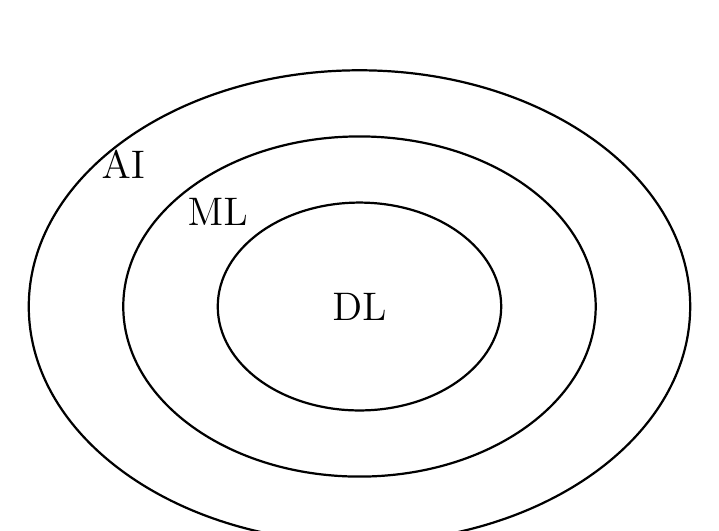
\begin{tikzpicture}[scale=1.2]
% 绘制三个相互嵌套的椭圆
\draw[thick] (0,0) ellipse (3.5cm and 2.5cm);
\draw[thick] (0,0) ellipse (2.5cm and 1.8cm);
\draw[thick] (0,0) ellipse (1.5cm and 1.1cm);

% 添加标签
\node at (-2.5,1.5) {\Large AI};
\node at (-1.5,1) {\Large ML};
\node at (0,0) {\Large DL};
\end{tikzpicture}
\caption{AI、ML和DL之间的关系}
\label{fig:ai_ml_dl_venn}
\end{figure}

AI指的是具有类人智能的系统。虽然机器学习是AI系统的关键组成部分,但还涉及其他要素。自动驾驶汽车是AI的原型例子。让我们仔细看看这样一个系统的设计(见图\ref{fig:self_driving_car})。汽车配备了摄像头,可以拍摄前方道路的实时图像/视频。然后将这些帧传递给执行\term{语义分割}{Semantic Segmentation}的机器学习算法,即分割出帧的不同区域并对每个区域中的对象类型(汽车、树、道路、天空等)进行分类。一旦完成这种分割,就将其传递给决策系统,该系统基于这个分割图像决定汽车的下一个动作应该是什么。然后这个信息通过控制模块,实际控制汽车的机械动作。整个过程模拟了真实驾驶员的行为,因此是人工智能。

\begin{figure}[H]
\centering
\begin{tikzpicture}[node distance=2cm, auto]
% 定义节点样式
\tikzstyle{block} = [rectangle, draw, fill=blue!20, text width=2cm, text centered, minimum height=1cm]
\tikzstyle{line} = [draw, -latex']

% 绘制流程图
\node [block] (camera) {摄像头};
\node [block, right of=camera] (segmenter) {语义分割器};
\node [block, right of=segmenter] (decision) {决策系统};
\node [block, right of=decision] (control) {控制模块};

% 连接节点
\path [line] (camera) -- (segmenter);
\path [line] (segmenter) -- (decision);
\path [line] (decision) -- (control);

% 添加标签
\node [below of=camera, node distance=1cm] {实时图像};
\node [below of=segmenter, node distance=1cm] {分割图像};
\node [below of=decision, node distance=1cm] {动作决策};
\node [below of=control, node distance=1cm] {机械控制};
\end{tikzpicture}
\caption{自动驾驶汽车AI系统示意图}
\label{fig:self_driving_car}
\end{figure}

另一方面,机器学习(ML)是该系统中使用数据训练的组件。也就是说,它们通过数据学习。在上面的例子中,语义分割器就是这样一个系统。有许多机器学习算法可以使用数据执行这项任务,我们将在本课程中学习其中的一些。决策系统也可能是ML组件——在这里,要做出的适当决策是从先前的数据中学到的。然而,它也可能是基于规则的非ML专家系统。

深度学习是机器学习算法的一个子集。最简单形式的深度学习架构,称为\term{前馈网络}{Feed-forward Network},包含多个非线性变换层。这种架构松散地受到信号如何在生物体的中枢神经系统中传输的启发。我们将在第2章更详细地研究深度学习架构。

\section{机器学习与计算物理}
\label{sec:ml_cp_combination}

现在我们对计算物理和机器学习有了更好的理解,下一个显而易见的问题是"我们为什么需要看两者的结合?"我们在下面列出几个动机:

\begin{itemize}
\item 对于"物理"数据的复杂模式,机器学习提供了表示数学定律的替代途径。考虑包含两个重要组件的物理过程。其中,一个得到很好理解并具有可信的数学模型,另一个理解不充分且没有数学描述。在这种情况下,可以对第一个组件使用计算物理,对第二个组件使用机器学习。这方面的具体例子是受能量守恒和复杂本构模型支配的系统。对于前者,我们可能有一个很好理解的数学模型,而对于后者,我们可能必须依赖机器学习来开发模型。

\item 机器学习通常非常依赖数据。但物理知识可以帮助限制输入和解/预测所在的\term{流形}{Manifold}。有了这样的约束,我们可以减少训练机器学习算法所需的数据量。

\item 用于分析计算物理的工具(\term{泛函分析}{Functional Analysis}、数值分析、精确解收敛的概念、概率框架)可以转移到机器学习中。将这些工具应用于机器学习有助于我们更好地理解和设计更好的机器学习算法。
\end{itemize}

我们简要总结本课程将涵盖的各种主题:

\begin{itemize}
\item \term{深度神经网络}{Deep Neural Networks}(多层感知器)及其收敛性。
\item \term{随机梯度下降}{Stochastic Gradient Descent}及其与常微分方程的关系。
\item \term{残差网络}{Residual Networks, ResNets}及其与非线性常微分方程的联系(\term{神经常微分方程}{Neural ODEs})。
\item \term{卷积神经网络}{Convolutional Neural Networks}及其与偏微分方程的联系。
\item 用于求解偏微分方程的深度学习算法。
\item 用于逼近算子的深度学习算法。
\item \term{生成算法}{Generative Algorithms}及其与计算物理的联系。
\item 用于求解概率反问题的生成算法。
\end{itemize}

\section{计算练习}
\label{sec:computational_exercises}

为了有效使用本课程中讨论的各种机器学习算法并解决计算练习,需要很好地掌握Python编程和PyTorch。下面列出了关于必要编程概念的各种资源和教程。

\begin{enumerate}
\item \textbf{Python基础、NumPy和绘图:}对于那些从未使用过Python的人,或者甚至对于那些熟悉Python并想要更新编程知识的人来说,一个很好的资源是\url{https://www.w3schools.com/python/}。本教程涵盖了重要的Python模块,如NumPy、Pandas和SciPy,描述了如何使用Matplotlib生成图表,以及如何读/写文件。

\item \textbf{PyTorch:}本课程中使用的代码将使用PyTorch编写,这是一个最初由Meta AI开发的机器学习框架。您可以按照这里给出的说明在您的机器上本地安装PyTorch:\url{https://pytorch.org/get-started/locally/}。关于使用PyTorch的各种教程可以在这里找到:\url{https://pytorch.org/tutorials/}。

\item \textbf{Google Colab:}如果您不希望在本地安装PyTorch,或者没有适当的硬件来训练深度学习模型,您也可以使用Google Colab:\url{https://colab.research.google.com}。Colab本质上是Jupyter notebook和Google Drive的组合,只需要您有一个Google账户。Colab吸引人的地方在于它预装了许多有用的包(如NumPy、PyTorch等),所以每个人都可以使用它而无需担心安装正确版本的库和依赖项。此外,它完全在云端运行,可以直接通过Web浏览器启动和使用。它还提供对强大GPU和TPU的免费访问。
\end{enumerate}

\subsection{环境设置建议}
\label{subsec:environment_setup}

对于初学者,我们建议按照以下顺序学习:

\begin{enumerate}
\item 首先熟悉Python基础语法和NumPy数组操作
\item 学习Matplotlib进行数据可视化
\item 了解PyTorch张量的基本操作
\item 学习如何构建和训练简单的神经网络
\item 实践本书中的编程练习
\end{enumerate}

\section{小结}
\label{sec:summary}

本章介绍了深度学习和计算物理领域的基础概念。我们探讨了:

\begin{itemize}
\item 计算物理的基本方法论及其在科学问题求解中的作用
\item 机器学习的不同类型及其应用领域
\item 人工智能、机器学习和深度学习之间的层次关系
\item 将机器学习与计算物理相结合的动机和潜在优势
\item 本课程将涵盖的主要主题概览
\end{itemize}

在接下来的章节中,我们将深入探讨深度神经网络的数学基础,学习各种训练技术,并将这些方法应用于具体的物理问题。我们将看到机器学习如何为传统的计算物理方法提供新的视角,以及物理直觉如何帮助我们设计更好的机器学习算法。

\newpage
\chapter{深度神经网络简介}

\section{多层感知机(MLP)结构}
MLP 的目标是近似函数 $f: \mathbb{R}^d \to \mathbb{R}^D$。其基本单元是人工神经元,由若干层堆叠组成。

\begin{mycomment}
在这一部分,我发现 MLP 的结构与“线性代数中的仿射变换 + 非线性函数”非常类似。  
可以把它理解为“线性映射 + 激活函数”的交替堆叠。  
\end{mycomment}

\newpage

\chapter{残差神经网络}

\section{深层网络的梯度消失}

\section{ResNets}

\section{与常微分方程的联系}

\section{神经 ODEs}

\newpage

\chapter{卷积神经网络}

\section{函数与图像}

\section{函数卷积}
\subsection{例 1}
\subsection{例 2}

\section{离散卷积}

\section{与有限差分近似的联系}

\section{卷积层}
\subsection{平均池化与最大池化}
\subsection{多通道输入的卷积}

\section{卷积神经网络(CNN)}

\section{转置卷积层}

\section{上采样}

\section{图像到图像的变换}

\section{计算练习:卷积神经网络}

\newpage

\chapter{用神经网络解偏微分方程}

\section{有限差分方法}

\section{谱配置方法}

\section{物理约束神经网络(PINNs)}

\section{推广到更一般的 PDE}

\section{PINNs 的误差分析}

\section{基于 PINNs 的数据同化}

\section{现有的 PINN 公式}

\section{计算练习:PINNs}

\newpage

\chapter{算子网络}

\section{参数化 PDEs}

\section{算子}

\section{深度算子网络(DeepONet)结构}
\subsection{DeepONet 的训练}
\subsection{DeepONet 的误差分析}

\section{物理约束 DeepONets}

\section{DeepONets 及其应用}

\section{傅里叶神经算子(FNO)}
\subsection{FNO 的离散化}
\subsection{傅里叶变换的应用}

\section{变分模仿算子网络(VarMiON)}
\subsection{背景}
\subsection{VarMiON 结构}
\subsection{VarMiON 的训练}
\subsection{VarMiON 近似的误差估计}

\section{网格图网络(MGNs)}
\subsection{背景}
\subsection{MGN 结构}
\subsection{MGN 的训练}

\section{计算练习:DeepONets}

\newpage

\chapter{生成式深度学习}

\section{生成算法}

\section{概率论入门}
\subsection{随机变量}
\subsection{累积分布函数}
\subsection{概率密度函数}
\subsection{常见随机变量举例}
\subsection{期望与方差}
\subsection{随机向量}
\subsection{联合概率密度函数}
\subsection{常见随机向量举例}
\subsection{期望与协方差}
\subsection{边缘分布与条件分布}

\section{纯生成问题}
\subsection{GANs}
\subsection{基于得分的扩散模型}

\section{条件生成算法}
\subsection{条件 GANs}
\subsection{条件扩散模型}

\newpage


% ---------- 参考文献(可选) ----------
\bibliographystyle{plain}
\bibliography{refs}

\end{document}
